\documentclass{article}
\usepackage{spconf,amsmath,amssymb,booktabs,multirow,url,graphicx}
\usepackage[hidelinks]{hyperref}
\urlstyle{same}

\title{WHEN DOES LEAVE-ONE-OUT SUFFICE?\\
AUDITING MINIMAL-CAUSE ATTRIBUTION IN RAG}
\name{Qing Lin$^{1}$, Long Zhang$^{2}$, Xudong Zhang$^{3,*}$}
\address{$^{1}$Dalian University of Technology\\
$^{2}$Inspur Cloud Information Technology Co., Ltd., Jinan, Shandong, China\\
$^{3}$Institute of Software, Chinese Academy of Sciences, Beijing, China\\
\texttt{linq@mail.dlut.edu.cn}; \texttt{zlong@ios.ac.cn}; \texttt{zhangxd20@ios.ac.cn}\\
\footnotesize ORCID: 0009-0007-5508-3404; 0000-0002-8979-7014; 0009-0005-0451-7810
\quad $^{*}$Corresponding author}

\begin{document}
\ninept
\maketitle

\begin{abstract}
RAG attribution is often scored per document although a response may have
several alternative minimal causes. We formalize attribution as enumeration of
all inclusion-minimal sufficient document sets and prove a boundary for
grand-coalition leave-one-out (LOO): under monotone replay, LOO recovers the
unique cause but returns only the intersection of alternatives. We introduce
fully oracled unique/alternative/non-monotone (U/A/N) strata and audit black-box
procedures on HotpotQA and Natural Questions with two 7B generators. Mask counts
overstate cost when masks render to identical prompts; correct prompt-level
caching removes an apparent advantage of a RAG-specific adaptation over
standard enumeration. An enumerate-first prompt-uniform residual audit preserves
perfect U/A recovery and raises source-clustered raw-N violation recall from
.388 to .952, but a no-collapse stress test falls to .814. We prove uniform
sampling minimax for an adversarial static hidden-witness subproblem. A frozen
geometry-aware ordering subsequently fails its prespecified holdout gate. Thus a
finite unviolated trace is diagnostic, not a monotonicity certificate.
\end{abstract}

\begin{keywords}
retrieval-augmented generation, context attribution, sufficient causes,
leave-one-out, evaluation audit
\end{keywords}

\section{Introduction}

RAG combines parametric generation with retrieved evidence
\cite{lewis2020rag,karpukhin2020,izacard2021}, but attribution still asks which passages caused a fixed
answer.
Existing methods assign document scores or citations
\cite{contextcite,mirage,selfcite}, but a scalar ranking does not identify a
\emph{set} of alternative minimal sufficient causes. This distinction matters in
poisoning and forensic analysis: removing one path can leave another intact.
Minimal sufficient subsets are established in explanation research
\cite{carter2019,ignatiev2019,marquessilva2021}; our question is narrower: what can exact
black-box replay establish for a fixed RAG context?

\textbf{Contributions.} We make four contributions. (1) \emph{Identifiability:}
we prove that LOO exactly recovers a unique monotone cause but only the common
backbone of alternatives, and that an unviolated finite trace is not a
monotonicity certificate. (2) \emph{Benchmarking:} we construct fully enumerated
U/A/N strata whose labels come from the realized generator truth table, never
the planted template. (3) \emph{Methodology:} we introduce an enumerate-first
pipeline that protects all-cause search, deduplicates byte-identical rendered
prompts, and spends only the residual physical-call budget on safety auditing;
uniform class sampling is minimax in a static hidden-witness game. (4)
\emph{Audit evidence:} corrected accounting removes an apparent method
advantage; transfer, no-collapse stress, and two frozen holdout attempts expose
where the diagnostic succeeds and where it must abstain.

\textbf{Relation to prior work.} Sufficient-input subsets and rationale
benchmarks formalize local evidence \cite{carter2019,deyoung2020}, while delta debugging minimizes a
failure-inducing input \cite{zeller2002}. ContextCite fits a KernelSHAP
surrogate over context ablations \cite{contextcite,lundberg2017}; MIRAGE and
SelfCite instead use model internals or citation supervision
\cite{mirage,selfcite}. Our all-cause endpoint differs from feature ranking and
single-subset minimization \cite{ribeiro2016,ribeiro2018anchors,fong2017}. Explanation quality also depends
on the claim and evaluation target \cite{miller2019,lipton2018}; we therefore
make faithfulness assumptions explicit and prefer intervention-backed tests
\cite{jacovi2020,jain2019,wiegreffe2019,serrano2019,yeh2019,ghorbani2019,hooker2019}. Post-hoc local
surrogates can also be adversarially misleading \cite{slack2020}.
Its standard baseline follows the same
minimal/maximal duality used by MUS/MCS enumeration \cite{liffiton2016}.
Property testing can reject functions that are far from monotone
\cite{goldreich2000}; our trace proposition is narrower and makes no tolerant-
testing lower-bound claim.

\textbf{Data availability.} Code, benchmark manifests, and replay artifacts are
publicly available at \url{https://github.com/violetzxd/CoalitionTrace}.

\section{Problem Setup and Boundaries}

For documents $D=\{1,\ldots,n\}$, let $r(S)$ be the complete rendered chat
prompt (including the system message and generation marker) obtained by
keeping the observed version of documents in $S$ and their contrastive
replacement otherwise. Deterministic replay defines
$v(S)=\mathbb{1}[\operatorname{NEM}(g(r(S)))=\operatorname{NEM}(y_t)]$, where
NEM is a frozen normalization and exact-match rule: a format-only extractor
removes an ``Answer:'' prefix, later lines, and a trailing parenthetical before
standard lowercase/article/punctuation normalization. A set $C$ is an
inclusion-minimal sufficient cause (relative to the fixed model, decoder,
replacement, and target) when $v(C)=1$ and $v(C')=0$ for every
$C'\subsetneq C$. Let
$\mathcal{M}(v)$ contain all such causes. We evaluate exact cause-set match
(ACEM), cause-set precision/recall/F1, observed non-monotonicity, and replays.

\textbf{Proposition 1 (LOO boundary).}
Write $D_{-i}=D\setminus\{i\}$. If $v$ is monotone and $v(D)=1$,
grand-coalition LOO returns
\begin{equation}
 \{i:v(D_{-i})=0\}=\bigcap_{C\in\mathcal{M}(v)} C.
\end{equation}
Hence LOO returns an inclusion-minimal sufficient cause exactly in the unique
regime, $|\mathcal{M}(v)|=1$. With alternatives it returns only their common
backbone. The proof follows because every
sufficient set contains a minimal cause: deleting $i$ fails exactly when every
minimal cause contains $i$.

\textbf{Corollary (one-query ambiguity test).} Let $B$ be the LOO set above.
Under the same assumptions, $v(B)=1$ iff $|\mathcal{M}(v)|=1$. Thus at most
$n+2$ replays (full, $n$ deletions, and $B$) classify U versus A and recover the
U cause. If $B$ is sufficient it contains a minimal cause, which must equal the
intersection and hence every minimal cause; the converse follows from
Proposition~1. This certificate is invalid without monotonicity.

This motivates three oracle strata, all requiring $v(\emptyset)=0$ and $v(D)=1$:
U has monotone $v$ and one minimal cause; A has monotone $v$ and at least two;
N contains a Boolean cover-edge violation.

\textbf{Proposition 2 (trace non-certifiability).}
Assume a partial trace over exact rendered-prompt classes has a monotone
completion. If an entirely unqueried class represented by $x$ has either a
queried insufficient strict superset or a queried sufficient strict subset,
then a non-monotone completion produces the identical trace: assign every mask
in that whole unqueried class the opposite of the value forced by monotonicity.
Thus absence of an
observed violation cannot certify monotonicity for such a trace.

\textbf{Proposition 3 (static hidden-witness minimax).}
After a fixed prefix, suppose $M$ classes remain, exactly $K$ are immediate
witnesses, every non-witness returns one common miss, misses cannot create new
witnesses, and all $K$-subsets are admissible. Any randomized adaptive audit of
$b\leq M$ classes has worst-case detection at most
$V=1-\binom{M-K}{b}/\binom{M}{b}$; uniform sampling without replacement attains
$V$ for every witness set. Indeed, under a uniformly hidden $K$-set, any fixed
all-miss query set of size at most $b$ intersects it with probability at most
$V$, so averaging yields one instance no easier than $V$; uniform sampling has
that probability pointwise. In a real sequential audit, dynamic witnesses can
only make the fixed-prefix expression a lower bound, not a global minimax claim.

\section{Methodology}

Figure~\ref{fig:method} summarizes our five-stage procedure. The separation is
deliberate: cause recovery, violation detection, and certification are different
objectives. Safety queries never preempt the task-matched cause enumerator. The
procedure maintains three persistent objects: a prompt-class cache $H$, a set
$\widehat{\mathcal M}$ of verified minimal causes, and an exclusion frontier
$F$. Every returned cause is replay-checked for sufficiency and member
necessity; every safety decision is tied to an explicit comparable pair.

\begin{figure*}[t]
\centering
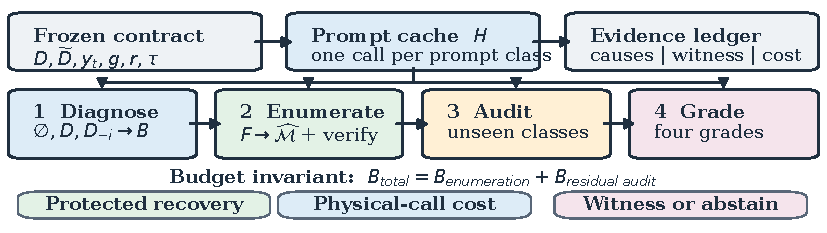
\includegraphics[width=.98\textwidth]{fig_method_overview.pdf}
\caption{CoalitionTrace methodology. Endpoint checks establish that the local
question is well posed. LOO gives a cheap backbone diagnostic; the exclusion
frontier searches all causes; residual unseen prompt classes are then audited.
Only an observed reversal rejects monotonicity---otherwise a non-exhaustive trace
abstains.}
\label{fig:method}
\end{figure*}

\textbf{Stage 1--2: validate, cache, and diagnose.} We first replay $\emptyset$ and $D$;
cases with $v(\emptyset)=1$ or $v(D)=0$ are out of scope. We then query every
$D_{-i}$, insert the resulting prompt classes into $H$, and form backbone $B$.
Under a justified monotonicity assumption,
$v(B)$ implements the corollary's U/A test; without that assumption it is only a
diagnostic fast path.

\textbf{Stage 3: protected all-cause enumeration.} At exclusion $E$, query the
maximal allowed set $D\setminus E$; prune if it is insufficient, otherwise
minimize it by deterministic single-document deletions to $C$, verify $C$, add
it to $\widehat{\mathcal M}$, and branch on $E\cup\{i\}$ for every $i\in C$.
Duplicate exclusions are removed and every replay first consults $H$. Branching
preserves a frontier entry disjoint from each undiscovered cause. Hence frontier
exhaustion is conditionally complete under monotonicity; budget exhaustion
returns discovered causes but abstains from completeness. This is a standard
minimal-explanation enumerator \cite{ignatiev2019,marquessilva2021}, not a new generic
enumeration result.

\textbf{Stage 4--5: residual audit and evidence grading.} The post-hoc wrapper
runs the enumerator unchanged, then samples previously unseen rendered-prompt
classes uniformly without replacement until the residual physical-call budget
is spent. After each replay, its value is propagated to every byte-identical
mask and compared with the observed subset closure. The audit stops at the first
pair $L\subset U$ with $v(L)=1,v(U)=0$. The grader then emits one of four states:
\emph{exact-monotone} (frontier and relevant closure exhausted),
\emph{conditional-complete} (frontier exhausted under monotonicity),
\emph{violated} (a concrete reversal exists), or \emph{budget-limited}. The
record bundles causes, witness, logical masks, unique prompts, tokens, stopping
reason, and cache multiplicities.

\textbf{Why the composition helps.} First, recovery is protected: the audit is
strictly residual, so adding it cannot lower U/A ACEM at the same total budget.
Second, exact prompt quotienting is cost-faithful and lossless for deterministic
replay, unlike semantic merging. Third, positive and negative conclusions are
intentionally asymmetric: one reversal is a sound refutation, whereas a clean
partial trace triggers abstention rather than a false certificate. Finally, the
output is auditable end to end---a reviewer can reconstruct each cause, cache
hit, cost, and safety label from the trace instead of trusting a scalar score.

\subsection{Exact replay accounting}

Define $S\sim T$ iff $r(S)=r(T)$ byte-for-byte. This is the conservative exact
request equivalence used by our cache, with model, decoder, scorer, and fixed
randomness held constant; token-ID equivalence could merge additional byte-
distinct prompts and is not claimed here.
\textbf{Proposition 4 (quotient accounting).} Any adaptive policy depending
only on its logical mask/response transcript can be simulated exactly with one
call per distinct class in $\mathcal{Q}=2^D/{\sim}$. Under $b$ uniform mask
draws, class $q$ is included with probability
$1-\binom{2^n-m_q}{b}/\binom{2^n}{b}$, biased by its multiplicity $m_q$.
For a \emph{static} single witness class, when its identity does not change and
every miss yields the same all-miss transcript, no adaptive policy using $c$
distinct class calls guarantees detection above $c/|\mathcal Q|$: inclusion
marginals sum to $c$, and class-uniform sampling attains the bound. Cache
induction, avoidance counting, and averaging prove the claims. The quotient is lossless for calls, not a cause lattice, so
queried values are propagated to all member masks before subset comparisons.

\section{Evaluation}

We ask whether LOO exhibits the predicted U/A boundary; whether prompt-level
accounting changes method comparisons; whether residual auditing improves
N-witness recall without sacrificing cause recovery; and whether development
gains survive transfer, no-collapse stress, and frozen holdouts.

\subsection{Benchmark and realized ground truth}

We start from public PoisonedRAG target questions \cite{poisonedrag} for
HotpotQA and Natural Questions \cite{yang2018hotpot,kwiatkowski2019nq}. Each $n=8$ context contains contrastive document
slots that instantiate one path (U), two disjoint or overlapping paths (A), or a
suppressor/restorer pattern (N). We exhaust all $2^8$ masks with greedy decoding.
We retain a source only when its realized table satisfies the exact stratum
definition; all failures and the screening funnel are retained in a hashed
artifact provided in the submitted supplementary material. A source query,
not a template or mask, is the sampling unit. The \emph{primary registry} frozen
test split contains 70 sources per dataset; later news, all-active, and holdout
audits use separately reported pools. Models are Qwen2.5-7B-Instruct and
Mistral-7B-Instruct-v0.3 at pinned revisions.

\subsection{Baselines, metrics, and protocol}

Methods are LOO; hierarchical deletion; ten-seed repeated greedy deletion; ten-
seed random masks; constrained KernelSHAP as a ContextCite-style surrogate;
a standard monotone exclusion enumerator; and a RAG adaptation that adds an LOO
backbone fast path. The post-hoc residual audit is evaluated separately from the
frozen seven-method comparison, with ten seeds. All share the same SHA-256 prompt cache. The primary small-$n$
budget is 48 unique prompts. Exact tables supply truth, not a deployable method.
We bootstrap source queries (10,000 resamples); stochastic seeds are averaged
within source and are never treated as samples. This intervention-based design
tests faithfulness directly rather than treating attention or plausibility as a
causal explanation \cite{jain2019,jacovi2020}; it also differs from training-data
influence analysis \cite{koh2017}.

\textbf{Oracle and construction validity.} Every stored table is checked for
all $2^n$ masks, target normalization, $v(\emptyset)$, and $v(D)$. Method-blind
selection keeps the first case in a frozen candidate order. An independent
implementation re-derived labels and causes for 224 candidate tables and found
zero mismatches. Planted templates are not truth: 79--90\% of realized A cases
contain a cause crossing planted paths, while only 4--21\% exactly match the
planted cause set. Cells contain two to at least four causes, of size one to
five; hence we score realized cause-set equality.

\textbf{Reproducibility and cost.} Model revisions, tokenizer chat templates,
case order, replacements, and greedy decoding (at most 16 new tokens) are
pinned. Each replay stores mask ID, raw/normalized answer, prompt SHA-256,
revision, tokens, and class size. The evaluator verifies sufficiency and
member-necessity against the exhaustive table; invalid subsets receive no
credit. Stochastic baselines use one fixed 10-seed panel.

\begin{table*}[t]
\caption{A-stratum ACEM / mean unique prompts at budget 48; $n_A$ is in
parentheses. Repeated and Random average ten seeds per source. StdEnum is the
task-matched standard enumerator; Adapt is its LOO-fast-path adaptation; Audit
adds prompt-uniform residual auditing and averages ten seeds.}
\label{tab:main}
\centering
\setlength{\tabcolsep}{2.2pt}
\begin{tabular}{llcccccc}
\toprule
Data & Model & LOO & Repeated & Random & StdEnum & Adapt & Audit \\
\midrule
Hotpot (58) & Qwen    & .00 (5.9) & .905 (13.0) & 1.00 (15.7) & 1.00 (12.4) & 1.00 (13.0) & 1.00 (15.7) \\
NQ (49)     & Qwen    & .00 (6.1) & .904 (14.2) & .920 (18.4) & 1.00 (14.2) & 1.00 (14.6) & 1.00 (18.4) \\
Hotpot (54) & Mistral & .00 (5.9) & .913 (13.1) & .981 (15.4) & 1.00 (11.9) & 1.00 (12.9) & 1.00 (15.4) \\
NQ (52)     & Mistral & .00 (5.9) & .931 (13.4) & .983 (15.8) & 1.00 (12.8) & 1.00 (14.1) & 1.00 (15.8) \\
\bottomrule
\end{tabular}
\end{table*}

\begin{figure*}[t]
\centering
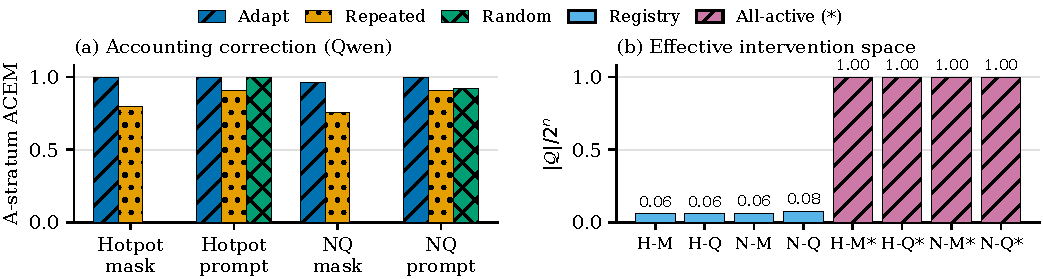
\includegraphics[width=.94\textwidth]{fig_audit.pdf}
\caption{The accounting audit. (a) A fixed 48-mask budget was wasted on
prompt-equivalent masks; charging unique rendered prompts sharply reduces the
apparent adaptation gap and rescues random masks. (b) Registry prompt spaces
collapse to a small fraction of the Boolean lattice, whereas the all-active
control has no literal prompt equivalence. Q/M denote Qwen/Mistral.}
\label{fig:audit}
\end{figure*}

\begin{figure}[t]
\centering
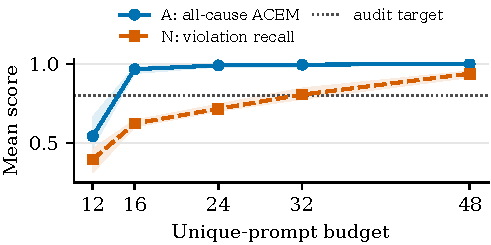
\includegraphics[width=.95\columnwidth]{fig_safe_frontier.pdf}
\caption{Post-hoc residual-audit budget frontier on four registry cells. Lines
are cell means; bands are cell minima--maxima. Cause enumeration is never
preempted, while residual budget improves violation recall.}
\label{fig:safe}
\end{figure}

\subsection{Attribution and accounting results}

\textbf{LOO has a sharp empirical boundary.} Across completed registry cells,
LOO obtains U ACEM 1.00 and A ACEM 0, exactly matching Proposition~1. The
standard enumerator and RAG adaptation obtain A ACEM 1.00 in the completed fair
cells. Hierarchical deletion and KernelSHAP also return at most one subset and
therefore have A ACEM 0 under the all-causes endpoint; this is an endpoint
mismatch, not evidence that their single returned subset is invalid.
On monotone A, every Adapt and StdEnum return is a member of the exhaustive
$\mathcal{M}(v)$ (cause precision 1.00; invalid-return rate 0 in all four cells).

\textbf{Correct caching collapses the claimed advantage.} In registry A cases,
the complete 256-mask tables contain only 15.7--19.8 distinct rendered prompts
on average (6.1--7.7\%). Under the original mask-count budget, the Qwen
adaptation exceeded repeated deletion by 20.5/20.2 ACEM points on Hotpot/NQ;
under unique-prompt accounting the gaps shrink to 9.5/9.6 points, below the
preregistered 10-point criterion. Random-mask ACEM changes from .00/.00 to
1.00/.920 because equivalent masks no longer consume fictitious generator
calls. With unique-prompt accounting,
Mistral A ACEM is 1.00 for the adaptation, .913/.931 for repeated deletion, and
.981/.983 for random masks on Hotpot/NQ. The standard enumerator matches 1.00
while using fewer prompts in every cell. These results reject the preregistered
method-superiority criterion and show that this A slice is close to saturated.
Source-level paired bootstraps give Adapt--Repeated gains (95\% intervals) of
.095 [.060,.136], .096 [.053,.149], .087 [.056,.122], and .069 [.042,.096] in
Table~\ref{tab:main} order; every point estimate is below the prespecified .10
margin. Adapt--StdEnum ACEM is exactly zero in every
cell (Holm-adjusted exact $p=1$). StdEnum saves .41--1.33 prompts on average;
the paired 95\% interval excludes zero in three cells and is
$[-.51,1.17]$ in NQ/Qwen. Ten stochastic seeds are averaged within each source.
The frozen news family replicates A ACEM 1.00 for both enumerators in all four
cells ($n=38$--53); repeated deletion is .898--.968 and random masks
.943--.976. NQ/Mistral has 38 rather than 40 sources and is descriptive. In a
post-hoc $n=10$ audit, only 1.7--2.1\% of 1,024 masks are distinct prompts and
both enumerators remain at 1.00. The all-active control instead has
$|\mathcal Q|=256$, but yields only 6/5/3/4 A sources and shifts many candidates
to N; it is a no-collapse stress test, not an accuracy benchmark.

\subsection{Safety-audit and generalization results}

\textbf{Residual auditing is diagnostic, not confirmatory.} StandardEnum already
observes violations in .267--.448 of raw N cases. Prompt-uniform residual Audit
raises ten-seed mean recall to .922--.980. Averaging model outcomes within each
dataset/source cluster gives .952 over 130 source clusters (222 model-cases;
bootstrap 95\% CI [.930,.972]) while retaining U/A ACEM 1.00. Witness soundness
implies no false flags, confirmed on all 429 monotone U/A model-cases. Its paired
gain over the identical enumeration prefix is .563 [.495,.630]. On detected N
cases, the witness appears after 4.05 residual prompt queries on average.
Figure~\ref{fig:safe} shows the
budget tradeoff: at 12,16,24,32,48 prompts, mean A ACEM is
.545,.967,.991,.995,1.00 and mean N recall is .421,.635,.734,.841,.949.

The wrapper was designed after inspecting the frozen comparison, so these are
explicitly post-hoc results. We freeze it for a post-hoc transfer check on the
separate news-wording family: N recall is .950 [.929,.968] over 123 clusters
(207 model-cases), and A ACEM remains 1.00. The all-active control, where
$|\mathcal{Q}|=256$, falls to .814 [.753,.869] over 75 clusters (142
model-cases);
this negative stress result prevents a near-certification interpretation.
Ablations also show that strategy novelty is limited: deterministic upward,
downward, and cover audits obtain .797, .667, and .935 on registry N, while a
randomized cover order gives .948. The robust benefit comes primarily from
protecting enumeration and spending the residual physical-call budget, not from
a uniquely superior boundary heuristic.

Offline replay of 1,000 uniform permutations per N case gives fixed-prefix
recall .920872 and sequential recall .920959 over 571 model-cases (138 source
clusters), a difference of .000087 [--.000030,.000495], with no dynamic-only
detection. This supports the static approximation only on this corpus.

We froze nearest ordering before a two-dataset/two-model holdout. Method-blind
selection retained 67/64 N cases in MSMARCO but only 15/16 in NQ, below the
30-per-cell floor. Descriptively, recall was .835 [.781,.886], with gains over
uniform of .038 [.004,.072] (below the .05 margin) and shuffled cover of .028
[--.009,.064]; one cell was negative. A separately preregistered feasibility
pilot on source-disjoint SQuAD and WebQuestions
data~\cite{rajpurkar2016squad,berant2013webquestions} also stopped before method
evaluation: N yields 14/13/19/14 all missed its 20-source floor; no final replay
or retuning followed. These blind failures accord with Proposition~3: geometry
may help under a validated distribution but cannot improve the adversarial
static guarantee. All methods make zero unconditional completeness claims on N;
by Proposition~2, an unviolated trace is inconclusive.

\section{Limitations and Conclusion}

The deployment rule is assumption-sensitive: validate $D$ and $\emptyset$;
under defensible monotonicity, use $v(B)$ to distinguish a unique cause from
alternatives, then enumerate. Otherwise only a reversal is decisive and a clean
partial trace abstains. Uniform class auditing is a small-$n$ method, and cost
must separate masks, unique prompts, and tokens. Results are local to constructed
contexts, fixed replacements, exact match, and two 7B models; they do not
estimate natural U/A/N prevalence. Nevertheless, they support a defensible
practice: protect all-cause search, audit only with residual budget, and never
promote an unviolated trace to a certificate. \textbf{AI use.} Codex assisted
code and editing; authors verified all claims.

\clearpage
\bibliographystyle{IEEEbib}
\bibliography{references}

\end{document}
